%% 由 build/emit_tex.py 生成（生成物，勿手改）；定制请放 user_style.tex / user_meta.yaml
\chapter{第 10 章 · Agent
工作流与验证方法}\label{ux7b2c-10-ux7ae0-agent-ux5de5ux4f5cux6d41ux4e0eux9a8cux8bc1ux65b9ux6cd5}

\section{01 Agent
工作流与核心能力}\label{agent-ux5de5ux4f5cux6d41ux4e0eux6838ux5fc3ux80fdux529b}

\begin{quote}
本节把 01
节的原理变成\textbf{可重复的操作习惯}：项目怎么给指令、任务怎么开场、权限怎么放、结果怎么验收。
配套图：子代理分工图（figures/10-agent-workflow/subagent\_split.png）；本节含一段可直接运行的
Python 代码。
\end{quote}

\subsection{本节目标}\label{ux672cux8282ux76eeux6807-33}

\begin{enumerate}
\def\labelenumi{\arabic{enumi}.}
\tightlist
\item
  会写一份最小可用的 AGENTS.md，让 Agent 不用每次重复问规范。
\item
  会用''计划先行 + 小步执行''的方式推进复杂任务。
\item
  掌握权限与审批的实践顺序：先只读、再放开、高风险动作单独确认。
\item
  会用\textbf{任务卡六件套}把一个模糊需求写成可验收的任务。
\item
  知道什么时候该派子代理、什么时候纯属浪费。
\end{enumerate}

\subsection{先修}\label{ux5148ux4fee-26}

\begin{itemize}
\tightlist
\item
  01 节（Agent 循环、上下文、权限、失败模式）；
\item
  02 节（已经装好 dsh，并能跑通第一个任务）。
\end{itemize}

\subsection{1.1
项目级指令：AGENTS.md}\label{ux9879ux76eeux7ea7ux6307ux4ee4agents.md}

\texttt{AGENTS.md} 是放在项目里的''常驻说明''，Agent
每次工作都会先读它。它解决的是\textbf{重复解释}问题：与其每次都说''读
CSV 要指定 UTF-8、图存到 output/、随机种子固定 42''，不如写进文件。

最小可用模板（复制到你的项目根目录即可）：

\begin{Shaded}
\begin{Highlighting}[]
\NormalTok{\#\# 项目说明}
\NormalTok{本项目是《Python 科学计算》课程的数据分析练习。}

\NormalTok{\#\# 环境}
\NormalTok{{-} Python 3.12，依赖见 environment.yml（numpy / pandas / scipy / statsmodels / scikit{-}learn / matplotlib）}
\NormalTok{{-} 运行命令统一用 python \textless{}脚本名\textgreater{}}

\NormalTok{\#\# 约定}
\NormalTok{{-} 读 CSV 一律显式指定编码 utf{-}8{-}sig，并先打印列名}
\NormalTok{{-} 随机过程必须固定种子：np.random.default\_rng(42)}
\NormalTok{{-} 输出文件放 output/，不覆盖 data/ 里的原始数据}
\NormalTok{{-} 中文图必须设置字体：Microsoft YaHei 或 SimHei}

\NormalTok{\#\# 质量要求}
\NormalTok{{-} 每个脚本末尾要有 assert 自检；改动后必须运行一次并贴出输出}
\NormalTok{{-} 不确定的地方先问我，不要擅自扩大改动范围}
\end{Highlighting}
\end{Shaded}

三条经验：

\begin{enumerate}
\def\labelenumi{\arabic{enumi}.}
\tightlist
\item
  \textbf{只写''会被违反''的约定}：写得越长越没人看，Agent 也一样；
\item
  \textbf{写清验收方式}：能让它自查的约定，比形容词有用；
\item
  \textbf{把 AGENTS.md 提交到 git}：它是项目的一部分，不是个人偏好。
\end{enumerate}

\subsection{1.2
计划先行：复杂任务先要计划}\label{ux8ba1ux5212ux5148ux884cux590dux6742ux4efbux52a1ux5148ux8981ux8ba1ux5212}

任务超过''改一个文件''的量级时，先让它进入\textbf{计划模式（Plan
mode）}，产出：要动哪些文件、分几步、每步怎么验证、有什么风险。你确认后再动手。

{\def\LTcaptype{none} % do not increment counter
\begin{longtable}[]{@{}ll@{}}
\toprule\noalign{}
任务规模 & 建议做法 \\
\midrule\noalign{}
\endhead
\bottomrule\noalign{}
\endlastfoot
一行改动、明确的小修 & 直接做，人审 diff \\
单文件重构、补测试 & 先说明要做什么，再执行 \\
多文件、跨目录、动数据 & \textbf{必须计划模式} + 你确认 \\
涉及删除、覆盖、联网安装 & 计划 + 逐条确认 \\
\end{longtable}
}

\begin{quote}
计划模式的价值不是''礼貌''，而是把\textbf{返工成本}从''改完发现方向错''降到''看计划发现方向错''。
\end{quote}

\subsection{1.3
会话与上下文管理}\label{ux4f1aux8bddux4e0eux4e0aux4e0bux6587ux7ba1ux7406}

\begin{itemize}
\tightlist
\item
  \textbf{一次会话只做一件事}：上下文里塞太多目标，它就容易抓错重点；
\item
  长任务定期收口，让它输出''已确认的结论 / 未解决的问题 /
  下一步''------这三行就是压缩后的上下文；
\item
  换任务就开新会话，把上一轮结论作为开场信息带过去；
\item
  会话记录是\textbf{证据链}：提交作业时把关键会话导出或截图留档。
\end{itemize}

\subsection{1.4
权限与审批：从小权限开始}\label{ux6743ux9650ux4e0eux5ba1ux6279ux4eceux5c0fux6743ux9650ux5f00ux59cb}

推荐的实践顺序（写进课程作业要求）：

\begin{enumerate}
\def\labelenumi{\arabic{enumi}.}
\tightlist
\item
  第一次接触项目：用 read-only，只让它解释；
\item
  确认它读懂了：切到 workspace-write，只在工作区内改；
\item
  涉及删除、批量重命名、装依赖、联网、访问工作区外目录：\textbf{逐条确认}；
\item
  任何情况下：不给它真实隐私数据，不让它接触你的 API Key 文件。
\end{enumerate}

高风险动作清单（看到就该停下来确认）：删除或覆盖文件、git
reset、批量替换、安装系统级软件、把数据上传到网络、修改环境变量。

\subsection{1.5
技能（skills）与工具（tools）}\label{ux6280ux80fdskillsux4e0eux5de5ux5177tools}

\begin{itemize}
\tightlist
\item
  \textbf{工具}是原子动作：读文件、写文件、跑命令、搜索；
\item
  \textbf{技能}是把''一组动作 +
  领域知识''打包好的工作流，例如''按模板生成实验报告''\,``批量处理
  Excel''。
\end{itemize}

判断标准：如果某套流程你会重复做三遍以上、且步骤固定，就值得写成技能（或一份模板文件
+ AGENTS.md 说明）。

\subsection{1.6
子代理：什么时候值得拆}\label{ux5b50ux4ee3ux7406ux4ec0ux4e48ux65f6ux5019ux503cux5f97ux62c6}

\begin{figure}
\centering
\pandocbounded{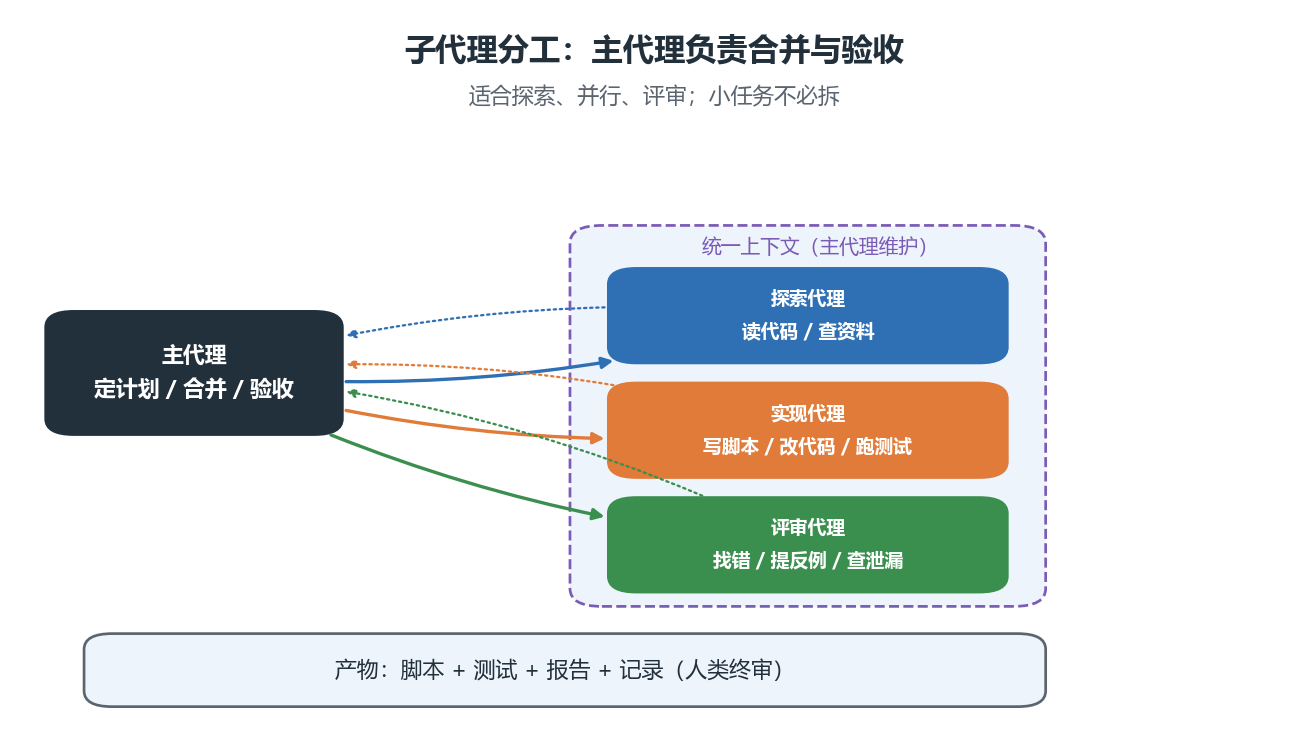
\includegraphics[keepaspectratio,alt={子代理分工}]{figures/10-agent-workflow/subagent_split.png}}
\caption{子代理分工}
\end{figure}

{\def\LTcaptype{none} % do not increment counter
\begin{longtable}[]{@{}
  >{\raggedright\arraybackslash}p{(\linewidth - 4\tabcolsep) * \real{0.3333}}
  >{\raggedright\arraybackslash}p{(\linewidth - 4\tabcolsep) * \real{0.3333}}
  >{\raggedright\arraybackslash}p{(\linewidth - 4\tabcolsep) * \real{0.3333}}@{}}
\toprule\noalign{}
\begin{minipage}[b]{\linewidth}\raggedright
场景
\end{minipage} & \begin{minipage}[b]{\linewidth}\raggedright
是否拆
\end{minipage} & \begin{minipage}[b]{\linewidth}\raggedright
原因
\end{minipage} \\
\midrule\noalign{}
\endhead
\bottomrule\noalign{}
\endlastfoot
先摸清陌生代码库，再决定怎么改 & 拆（探索代理） &
大量阅读会污染主上下文 \\
三个互不依赖的模块同时改 & 拆（并行） & 省时间 \\
关键结论需要第二双眼睛 & 拆（评审代理） & 专职找错，避免自我确认 \\
改一个函数、加一行日志 & 不拆 & 派发与合并的开销比任务本身还大 \\
\end{longtable}
}

\begin{quote}
记住：子代理不是''更强的模型''，而是\textbf{上下文隔离 +
角色分工}；每个子代理都会单独消耗 token。
\end{quote}

\subsection{1.7
验证驱动工作流（本节核心）}\label{ux9a8cux8bc1ux9a71ux52a8ux5de5ux4f5cux6d41ux672cux8282ux6838ux5fc3}

把任何任务写成\textbf{任务卡六件套}：

{\def\LTcaptype{none} % do not increment counter
\begin{longtable}[]{@{}lll@{}}
\toprule\noalign{}
要素 & 写什么 & 例 \\
\midrule\noalign{}
\endhead
\bottomrule\noalign{}
\endlastfoot
目标 & 一句话说清要达成什么 & 算出每个学生的平均分 \\
约束 & 不许动什么、用什么环境 & 只新增 scores\_fixed.py，不动 data/ \\
验收标准 & \textbf{可执行}的判据 & 长度 8、形状 (8,)、与手算一致 \\
证据 & 要它给出什么证明 & 运行输出 + 断言结果 \\
复核 & 人要检查哪几点 & 归一化是否逐列、排名是否带姓名 \\
提交 & 交付形态 & 文件 + 说明 + 会话记录 \\
\end{longtable}
}

\textbf{验收标准写法的正反例}：

{\def\LTcaptype{none} % do not increment counter
\begin{longtable}[]{@{}
  >{\raggedright\arraybackslash}p{(\linewidth - 2\tabcolsep) * \real{0.5000}}
  >{\raggedright\arraybackslash}p{(\linewidth - 2\tabcolsep) * \real{0.5000}}@{}}
\toprule\noalign{}
\begin{minipage}[b]{\linewidth}\raggedright
差的写法
\end{minipage} & \begin{minipage}[b]{\linewidth}\raggedright
好的写法
\end{minipage} \\
\midrule\noalign{}
\endhead
\bottomrule\noalign{}
\endlastfoot
结果要正确 & 平均分长度必须是 8，且与手算 {[}83.33, 65.0, \ldots{]}
一致 \\
图画得好看点 & 图保存到 output/trend.png；x 轴为小时、y
轴为温度（摄氏度）；标题含''传感器温度'' \\
检查有没有问题 & 用 assert
检查：行数守恒（清洗前后差值等于删除的重复行数）、缺失值策略已记录 \\
\end{longtable}
}

\textbf{为什么必须可执行}：只有可执行的判据才能被反复验证。看一个最小例子------同一段代码，两种
axis，只有一种能通过断言：

\begin{Shaded}
\begin{Highlighting}[]
\ImportTok{import}\NormalTok{ numpy }\ImportTok{as}\NormalTok{ np}
\NormalTok{np.set\_printoptions(precision}\OperatorTok{=}\DecValTok{2}\NormalTok{, suppress}\OperatorTok{=}\VariableTok{True}\NormalTok{)}
\NormalTok{scores }\OperatorTok{=}\NormalTok{ np.array([[}\DecValTok{82}\NormalTok{, }\DecValTok{90}\NormalTok{, }\DecValTok{78}\NormalTok{], [}\DecValTok{60}\NormalTok{, }\DecValTok{65}\NormalTok{, }\DecValTok{70}\NormalTok{], [}\DecValTok{95}\NormalTok{, }\DecValTok{88}\NormalTok{, }\DecValTok{92}\NormalTok{], [}\DecValTok{70}\NormalTok{, }\DecValTok{72}\NormalTok{, }\DecValTok{68}\NormalTok{]], dtype}\OperatorTok{=}\BuiltInTok{float}\NormalTok{)}

\KeywordTok{def}\NormalTok{ check\_student\_mean(m):}
\NormalTok{    m }\OperatorTok{=}\NormalTok{ np.asarray(m)}
    \ControlFlowTok{assert}\NormalTok{ m.shape }\OperatorTok{==}\NormalTok{ (}\DecValTok{4}\NormalTok{,), }\StringTok{"形状必须是 (4,)，每个学生一个平均分"}
    \ControlFlowTok{assert}\NormalTok{ np.allclose(m, scores.mean(axis}\OperatorTok{=}\DecValTok{1}\NormalTok{)), }\StringTok{"数值必须与手算一致"}
    \ControlFlowTok{return} \VariableTok{True}

\ControlFlowTok{for}\NormalTok{ axis }\KeywordTok{in}\NormalTok{ (}\DecValTok{0}\NormalTok{, }\DecValTok{1}\NormalTok{):}
    \ControlFlowTok{try}\NormalTok{:}
\NormalTok{        check\_student\_mean(scores.mean(axis}\OperatorTok{=}\NormalTok{axis))}
        \BuiltInTok{print}\NormalTok{(}\StringTok{"axis=}\SpecialCharTok{\%d}\StringTok{ {-}\textgreater{} 断言通过"} \OperatorTok{\%}\NormalTok{ axis)}
    \ControlFlowTok{except} \PreprocessorTok{AssertionError} \ImportTok{as}\NormalTok{ e:}
        \BuiltInTok{print}\NormalTok{(}\StringTok{"axis=}\SpecialCharTok{\%d}\StringTok{ {-}\textgreater{} 断言不通过：}\SpecialCharTok{\%s}\StringTok{"} \OperatorTok{\%}\NormalTok{ (axis, e))}
\end{Highlighting}
\end{Shaded}

\begin{Shaded}
\begin{Highlighting}[]
\NormalTok{axis=0 {-}\textgreater{} 断言不通过：形状必须是 (4,)，每个学生一个平均分}
\NormalTok{axis=1 {-}\textgreater{} 断言通过}
\end{Highlighting}
\end{Shaded}

\subsection{1.8
提示词写法清单}\label{ux63d0ux793aux8bcdux5199ux6cd5ux6e05ux5355}

\begin{enumerate}
\def\labelenumi{\arabic{enumi}.}
\tightlist
\item
  \textbf{说清目标与判据}，不要只说''帮我看看''；
\item
  \textbf{给最小复现}：能跑的 20 行，胜过 2000 行项目；
\item
  \textbf{限定范围}：明确''只改 X、不动 Y''；
\item
  \textbf{要求自证}：让它跑一次并贴输出，而不是''我觉得对''；
\item
  \textbf{要求打印中间量}：形状、量纲、前几行、统计量；
\item
  \textbf{一次只做一件事}：多个目标拆成多轮；
\item
  \textbf{不确定就问}：明确告诉它''信息不足时先提问，不要猜''。
\end{enumerate}

\subsection{1.9
一个完整示例：把''帮我改改''变成任务卡}\label{ux4e00ux4e2aux5b8cux6574ux793aux4f8bux628aux5e2eux6211ux6539ux6539ux53d8ux6210ux4efbux52a1ux5361}

\begin{Shaded}
\begin{Highlighting}[]
\NormalTok{【目标】修复 data/scores\_buggy.py 中"每个学生平均分"和"归一化"两处错误，产出 data/scores\_fixed.py。}
\NormalTok{【约束】只新增 scores\_fixed.py，不修改 data/scores.csv 与 scores\_buggy.py；使用现有 scicomp 环境。}
\NormalTok{【验收标准】}
\NormalTok{  1) student\_mean 的形状是 (8,)；}
\NormalTok{  2) 归一化逐列进行：norm.min(axis=0) 全为 0、norm.max(axis=0) 全为 1；}
\NormalTok{  3) 加权总分第一名是王五（91.4 分），且打印时带姓名。}
\NormalTok{【证据】贴出 python data/scores\_fixed.py 的完整输出，并给出三条 assert 的通过结果。}
\NormalTok{【复核】我会检查：是否动了原始数据、归一化是否逐列、排名是否真的排序（而不是取前三个）。}
\NormalTok{【提交】scores\_fixed.py + 运行输出 + 本次会话记录。}
\end{Highlighting}
\end{Shaded}

这份任务卡就是第 11 章四个案例的统一模板。

\subsection{本节小结}\label{ux672cux8282ux5c0fux7ed3-5}

\begin{enumerate}
\def\labelenumi{\arabic{enumi}.}
\tightlist
\item
  AGENTS.md 把''每次都要说的规范''变成项目文件；
\item
  复杂任务先计划、后执行、小步验证；
\item
  权限从小往大放，高风险动作逐条确认；
\item
  任务卡六件套：目标、约束、验收标准、证据、复核、提交；
\item
  验收标准必须\textbf{可执行}，否则等于没有。
\end{enumerate}

\subsection{思考题}\label{ux601dux8003ux9898-29}

\begin{enumerate}
\def\labelenumi{\arabic{enumi}.}
\tightlist
\item
  为什么''结果要正确''不算验收标准？请把它改写成两条可执行判据。
\item
  什么情况下应该派评审代理？它能替代你自己的复核吗？
\item
  上下文里放 AGENTS.md 有什么代价？什么时候该精简它？
\item
  你打算怎么把''会话记录''变成作业的一部分？
\end{enumerate}

\subsection{练习与延伸阅读}\label{ux7ec3ux4e60ux4e0eux5ef6ux4f38ux9605ux8bfb-2}

\begin{itemize}
\tightlist
\item
  练习：第 11 章 \texttt{exercises/} 第 6--8 题（审查题与任务卡题）；
\item
  上机：第 11 章 \texttt{lab/} Part A（审查预置产出物）；
\item
  下一章：第 11 章 01 案例一（读懂并修复 NumPy 代码）。
\end{itemize}

\newpage
